\let\mymarginpar\marginpar

\documentclass[11pt,twoside]{article}

%\long\def\authornote#1{%
%        \leavevmode\unskip\raisebox{-3.5pt}{\rlap{$\scriptstyle\diamond$}}%
%        \marginpar{\raggedright\hbadness=10000
%        \def\baselinestretch{0.8}\tiny
%        \it #1\par}}
%\newcommand{\ville}[1]{\authornote{NOTE TO SELF: #1}}

\marginparwidth=1cm
\marginparsep=5pt
\newcommand\ville[1]{%
    \mymarginpar{\raggedright\hbadness=10000\tiny\it #1\par}}


\usepackage{amsmath} 
\usepackage{times}
\usepackage{amsmath,amsthm,amssymb}
\usepackage{fancyhdr}
\usepackage{moreverb}
\usepackage{graphicx}
\usepackage{amssymb}
\usepackage{url}
\usepackage{multirow} 
\usepackage[boxed, section]{algorithm}
%\usepackage{algorithm}
\usepackage{algorithmic}
\usepackage{cite}
\usepackage{multirow} 
\usepackage{rotating}
\usepackage{geometry}
\usepackage{fix-cm}
%\usepackage{subfigure}
\usepackage{natbib}
\usepackage{caption}
\usepackage{subcaption}
\usepackage{color}

\renewcommand{\baselinestretch}{1.2}
\setlength{\topmargin}{-0.3in}
\setlength{\textwidth}{6in}
\setlength{\textheight}{8.5in}
\setlength{\oddsidemargin}{0.25in}
\setlength{\evensidemargin}{0.25in}
\raggedbottom




%\allowdisplaybreaks

% Math Macros.  It would be better to use the AMS LaTeX package,
% including the Bbb fonts, but I'm showing how to get by with the most
% primitive version of LaTeX.  I follow the naming convention to begin
% user-defined macro and variable names with the prefix "my" to make it
% easier to distiguish user-defined macros from LaTeX commands.
%
\newcommand{\myN}{\hbox{N\hspace*{-.9em}I\hspace*{.4em}}}
\newcommand{\myZ}{\hbox{Z}^+}
\newcommand{\myR}{\hbox{R}}
\renewcommand{\P}{\mathbb{P}}
\newcommand{\E}{\mathbb{E}}
\newtheorem{defi}{Definition}
\newtheorem{theorem}{Theorem}[section]
\newtheorem{lemma}[theorem]{Observation}
\newtheorem{observation}[theorem]{Observation}
\DeclareMathOperator*{\argmax}{arg\,max}

\theoremstyle{definition}
\newtheorem{example}[theorem]{Example}

\theoremstyle{definition}
\newtheorem{definition}[theorem]{Definition}


\newcommand{\myfunction}[3]
{${#1} : {#2} \rightarrow {#3}$ }

\newcommand{\myzrfunction}[1]
{\myfunction{#1}{{\myZ}}{{\myR}}}


\newcommand{\mysection}[1]
{\noindent {\bf {#1}}}

%%%%%% Begin document with header and title %%%%%%%%%

\begin{document}

\title{Principled Understanding of Probability Extremizing through Information Diversity}
%\title{A Novel Framework for Analyzing Subjective Response Data}
\author{
Ville A. Satop\"a\"a, Robin Pemantle, and Lyle H. Ungar\\
\\
 \small Department of Statistics\\
 \small The Wharton School of the University of Pennsylvania\\
 \small Philadelphia, PA 19104- 6340, USA\\ [-0.25in]} \date{}
\maketitle

\pagestyle{myheadings}
\markboth{Understanding Probability Extremizing}{Satop\"a\"a et al.}
\thispagestyle{empty}

\begin{abstract}
Randomness in scientific estimation is generally assumed to arise from
unmeasured or uncontrolled factors. However, when combining subjective probability estimates, heterogeneity
stemming from people's cognitive or information diversity is often
more important than measurement noise.  This paper presents a novel
framework that models the heterogeneity arising
from experts that use partially overlapping information sources, and applies that model to the task of
aggregating the probabilities given by a group of experts who forecast
whether an event will occur or not. Our model describes the
distribution of information across experts in terms of easily
interpretable parameters and shows how the optimal amount
of \textit{extremizing} of the average probability forecast (shifting
it closer to its nearest extreme) varies as a function of the experts'
information overlap.  Our model thus gives a more principled
understanding of the historically {\it ad hoc} practice of extremizing
average forecasts.
\end{abstract}



\section{Introduction}
Combining multiple probability forecasts is an important problem with many applications including medical diagnosis (\cite{wilson1998prediction, pepe2003statistical}), political and socio-economic foresight (\cite{tetlock2005expert}), and meteorology (\cite{sanders1963subjective, vislocky1995improved, baars2005performance}). There is strong empirical evidence that bringing together the strengths of different experts by combining their probability forecasts into a single consensus, known as the \textit{crowd belief},  improves predictive performance (\cite{clemen1989combining, armstrong2001combining}). To illustrate, consider two experts $E_1$ and $E_2$ who know, say, respective 25\% and 10\% of all information that is relevant to a forecasting problem. If each expert knows something that the other expert does not, some combination of their probability forecasts is likely to be more informed than either one of the individual probabilities. The naive approach is to simply average the individual forecasts.  Given that $E_1$'s forecast is more informed and therefore typically closer to the actual outcome of the event ($0.0$ if the event does not happen and $1.0$ if it happens), it should be weighted more heavily than $E_2$'s forecast. The simple average, however, gives each forecasts equal weight. The result is an aggregate probability that is often under-confident, i.e. too close to 0.5. This is formalized in \cite{Ranjan08} who explain that if the aggregate is linear, the group is necessarily under-confident.


Many previous developments suggest that shifting the average probability closer to its nearest extreme (0.0 or 1.0), known as \textit{extremizing}, yields improved forecasting performance. For instance, \cite{satopaa} use a logistic regression model to derive an extremizing aggregator that performs well in practice. \cite{Ranjan08} propose transforming the average probability with the cumulative distribution function (CDF) of a beta distribution. If both the shape and scale of this beta distribution are equal and constrained to be at least 1.0,  the aggregator extremizes and has some attractive theoretical properties (\cite{Wallsten2001}).  \cite{Baron} give two intuitive justifications for extremizing and discuss an aggregator that has been previously used by \cite{Erev1994, shlomi2010subjective}, and even \cite{karmarkar1978subjectively}. In a related empirical study, \cite{mellers} show that extremizing can improve the quality of aggregate probability forecasts of international events. The benefits of extremizing have also been acknowledged by many other investigators (see, e.g., \cite{turner2013forecast, Ariely00theeffects}).

Unfortunately, the existing aggregators have several drawbacks. First, they are based on \textit{ad hoc} techniques that typically learn the amount of extremizing by optimizing a scoring rule over a separate training set (see \cite{Gneiting04strictlyproper} for a discussion on scoring rules). Given that this requires several events or at least repeated realizations of a single event, it is not clear how appropriate these aggregators are for combining forecasts of a one-time event. 
%Such single event aggregation requires a model that naturally yields extremizing.
%It is concerning that extremizing does not arise naturally from the underlying model. 
Second, the aggregators generally provide very little insight beyond the aggregate probability. Therefore it is still not well-understood when and how much extremizing should be performed. 


These drawbacks are largely due to the modelers' inability to setup a feasible framework that aligns with the psychological environment of probability forecasting. Many aggregators are based on the \textit{classical measurement error model} under which each forecast is considered equal to the true value plus some mean-zero idiosyncratic noise. Therefore forecast heterogeneity is assumed to arise from a probability distribution. This model, however, cannot fully explain how experts assign probabilities to complex world events (\cite{parunak2013exploiting}). According to \cite{hong2009interpreted} the classical measurement error model can result in misleading information aggregation and strategic choices in situations that involve interpreted forecasts. They define a forecast to be ``interpreted" if the expert forms it based on a personal interpretation of (a subset of) factors or cues that influence the target event. Therefore, as different interpretations lead to different beliefs, forecast heterogeneity is assumed to stem from ``cognitive diversity" instead of a probability distribution. This work has been analyzed and extended in many other settings. For instance, \cite{parunak2013characterizing} demonstrate that interpreted forecasts require aggregation techniques such as voting that can leave the convex hull of the individual forecasts. \cite{broomell2009experts} analyze inter-expert correlation under the assumption that the cues can be mapped to the experts' forecasts via different linear regression functions. Unfortunately, any previous work on interpreted forecasts has only produced abstract concepts and still lacks a formal model with quantitative predictions. 

%The main problem is that it is not clear how ``cognitive diversity" can be measured in complex real-world situations.

The first contribution of this paper develops a concrete model for probability forecasts. The model is based on the \textit{partial information framework} that assumes experts with different levels of access to information sources such as newspapers, people, websites, photographs, and even languages. Knowing all information would deterministically reveal the final outcome of the target event. The experts, however, observe and make probability forecasts based on different subsets of the full information. Therefore forecast heterogeneity stems from information diversity. This gives results that often agree with previous work on interpreted forecasts while permitting models that can be potentially estimated in practice. For instance, our model for probability forecasts represents  the experts' information with a covariance matrix that can be constrained and estimated in different ways to suit the available resources. 

The second contribution of this paper provides novel direction in overcoming the aforementioned drawbacks of the current aggregators. The first step is to derive a probability aggregator based on the partial information model. This aggregator depends on the information structure among the experts. Therefore it establishes a link between the amount of extremizing of naive aggregates, such as the average probit- and logit-forecasts, and the information among the experts. This improves our understanding of extremizing. In particular, our analysis reveals two main causes of \textit{reverse-extremizing} (shifting the average probability away from its closest extreme). These sources lead us to a group of information structures that are immune to reverse-extremizing. The corresponding aggregator always extremizes and can leave the convex hull of the individual forecasts. It depends on two parameters that can be interpreted as the average amount of information known by an expert and the average amount of information shared between any two experts. Given that these two quantities can be directly estimated from the experts' forecasts, the aggregator is appropriate for combining forecasts of a one-time event. 


\textcolor{red}{Make it clear that the second aggregator is a sub case of the first}
\textcolor{red}{Is it clear what information structure means. Maybe add an example}
\textcolor{red}{Make sure that is actually can leave the convex hull}
\textcolor{red}{Split into two contributions: understanding extemizing, and offering a aggregator that can work on one-time events}


%The amount of extremization performed by this aggregator has a simple form that can be studied graphically.


%This leads to an aggregator that always extremizes, depends only on two interpretable parameters, and hence  can be learned from the experts' forecasts without a separate training set.

%This leads an information structure that is immune to both sources of reverse-extremization. The corresponding aggregator always extremizes and depends only on two intuitive parameters that can be learned from the experts' forecasts without a separate training set. The amount of extremization performed by this aggregator has a simple form that is studied graphically at the end of Section 3.


%structures that make any particular aggregation procedure, such as averaging or voting, work well in practice. 

%Under a simplified information structure this expressions depends only on three intuitive parameters. This allows us to visualize extremization and make concrete statements on when and how much extremization should be performed. 




This paper begins in Section 2 by introducing the partial information model for probability forecasts. Section 3 develops the aggregator based on this model, gives a closed-form expression for the amount of extremizing under different information structures, and studies aggregation under unstructured, non-overlapping, and compound symmetric information. Section 4 relates some of the main results to our past experience with real-world forecasting data, discusses model limitations, and describes potential future directions. 



%List out subjective/qualitative data sources
% 1. Economic forecasts
%.2. Online ratings
% 3. Sports or performance scores
% 4. Property valuation
% 5. Patient diagnosis
% 6. 

%An easy way to remember this distinction is to think of objective measurements and quantitative research as describing physical objects with numerical quantities and to think of subjective data and qualitative research as phenomenological experience partially dependent on the subject observing and in need of his or her qualifications to be made full sense of.
%http://adamschwartz.hubpages.com/hub/The-Difference-Between-Objective-and-Subjective-Data


\section{Model for Probability Forecasts}
\label{Model}
This section derives a \textit{partial information model} for probability forecasts made by a group of experts who aim to forecast whether a binary event will occur or not. The first step is to consider a probability space  $(\Omega, \mathcal{F}, \P)$, where the set $\Omega$ contains all possible states of the world,  $\mathcal{F}$ is a $\sigma$-field of all subsets of $\Omega$, and $\P$ is a probability measure. Let $S = [0,1]$ denote the unit interval and, on the probability space $(\Omega, \mathcal{F}, \P)$, define a Gaussian process $\{ X_B \}$ that is indexed by Borel measurable subsets $B \in S$. Endow the unit interval $S$ with the uniform measure $\mu$ such that the Gaussian process has a covariance structure $\text{cov}(X_B, X_{B'}) = \mu(B \cap B') = |B \cap B'|$, i.e. the length of the intersection. This process provides the pool of information that is central to the partial information model. The target event is defined as $A = \{ X_{S} > 0\}$. Even though the pool of information is indexed by the unit interval, it is important to emphasize that there is no sense of time or ranking of information. Instead the pool is a collection of information, where each piece of information has \textit{a priori} an equal chance to contribute to the final outcome of the event. It is not necessary to assume anything about the source or form of the information. For instance, the information may stem from photographs, survey research, books, or even interviews. All these details have been abstracted away. Instead any single piece of information is completely characterized by its effect on the target event. 



It is helpful to begin the introduction by considering only two experts. Assume that experts $E_1$ and $E_2$ see respective $\delta_1$ and $\delta_2$ portions of the Gaussian process. These portions form their information sets. The overlap in their information sets is a fixed share $\rho$ of what is seen by either expert. Therefore, if $I_1, I_2 \subseteq S$ denote the information sets observed by $E_1$ and $E_2$, respectively, then
\begin{align*}
\mu(I_1) = |I_1| &= \delta_1\\
\mu(I_2) = |I_2| &= \delta_2\\
\mu(I_1 \cap I_2) =  |I_1 \cap I_2| &= \rho
\end{align*}
\begin{figure}[htbp]
%   \hspace{-2em}
   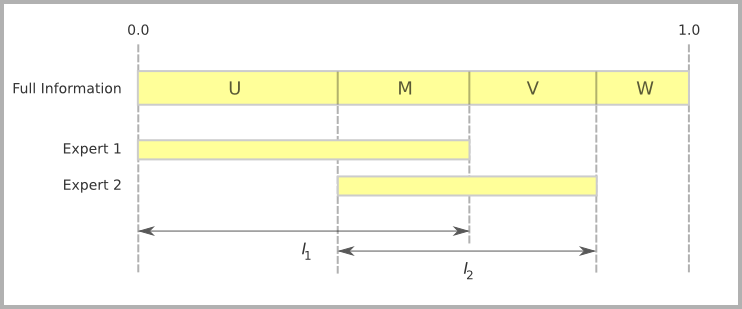
\includegraphics[width = \textwidth]{N=2} % requires the graphicx package
   \caption{Illustration of the partial information model with two experts.}
   \label{diagram2}
\end{figure}
Figure \ref{diagram2} illustrates this setup. In this diagram the Gaussian process has been partitioned into four parts based on the experts' information sets:
\begin{align*}
 U &= X_{I_1 / I_2}
& M &= X_{I_1 \cap I_2}\\
 V &= X_{I_2 / I_1}
& W &= X_{(I_1 \cup I_2)^c}
\end{align*}
Then,
\begin{align*}
X_{I_1} &= U + M\\
X_{I_2} &= M + V\\
X_S &= U+M+V+W,
\end{align*}
where $U, V, M, W$ are independent Gaussians with respective variances $\delta_1-\rho$, $\delta_2-\rho$, $\rho$, $1+\rho-\delta_1 - \delta_2$. The random variable $X_{I_j}$ can be interpreted as the information known by $E_j$. The joint distribution of $X_{S}$, $X_{I_1}$, and $X_{I_2}$ is a multivariate normal distribution. That is,
\begin{align}
\left(\begin{matrix} X_S \\ X_{I_1}\\ X_{I_2} \end{matrix}\right) &\sim \mathcal{N}\left(
 \boldsymbol{0},  \left(\begin{matrix} 
1 & \delta_1 & \delta_2\\
\delta_1 & \delta_1 &\rho\\
\delta_2 & \rho & \delta_2
 \end{matrix}\right)\right) \label{twoExperts}
\end{align}
Given that $X_S$ has mean zero, $\P(X_S > 0) = \P(A) = 0.5$. This can be viewed as the decision maker's prior probability of $A$ and is easily adjusted by changing the event $A$. More specifically, if the decision maker's prior belief is denoted with $\tilde{p}$, the event $A$ should be defined as $A = \{ X_S > \Phi^{-1}(1-\tilde{p}) \}$, where $\Phi$ represents the standard Gaussian CDF. As this paper is not concerned with any particular problem, the prior belief is taken non-informative, i.e. $\tilde{p} = 0.5$.  

\begin{figure}[htbp]
   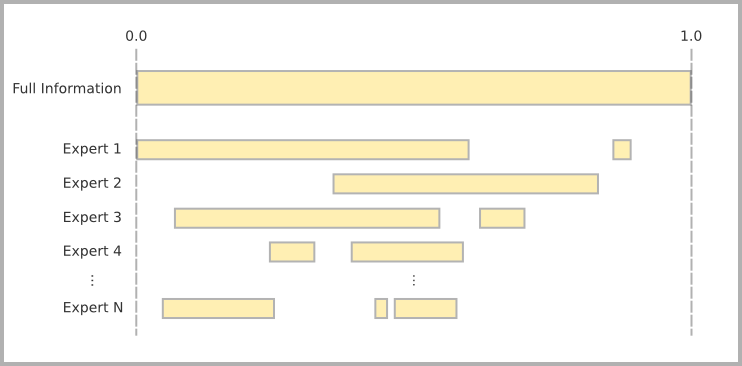
\includegraphics[width = \textwidth]{N=N} % requires the graphicx package
   \caption{Illustration of the partial information model with $N$ experts.}
   \label{diagramN}
\end{figure}



Consider now $N$ experts. Let $|I_j| = \delta_j$ be the amount of information known by expert $E_j$, and $|I_i \cap I_j| = \rho_{ij}$ be the information overlap between experts $E_i$ and $E_j$. Expression (\ref{twoExperts}) generalizes to the vector $(X_{S}, X_{I_1}, X_{I_2}, \dots, X_{I_N})$ as follows.
\begin{align}
\left(\begin{matrix} X_S \\ X_{I_1}\\ \vdots \\ X_{I_N} \end{matrix}\right) &\sim \mathcal{N}\left( \left(\begin{matrix} 
\mu_1 \\ \boldsymbol{\mu}_2
 \end{matrix}\right) =
 \boldsymbol{0}, \left(\begin{matrix} 
\Sigma_{11} & \Sigma_{12}\\
\Sigma_{21} & \Sigma_{22}\\
 \end{matrix}\right) 
 =
 \left(\begin{array}{c | c c cc }
1 & \delta_1 & \delta_2 & \dots & \delta_N  \\ \hline
\delta_1 & \delta_1 &\rho_{1,2} & \dots & \rho_{1,N}   \\ 
\delta_2 & \rho_{2,1} & \delta_2 & \dots & \rho_{2,N}  \\ 
\vdots & \vdots & \vdots & \ddots & \vdots  \\ 
\delta_N & \rho_{N,1} & \rho_{N,2} & \dots & \delta_N\\ 
 \end{array}\right)\right)  \label{NExperts}
\end{align}
This case is illustrated in Figure \ref{diagramN}. It is important to notice that $I_j$ does not have to be a contiguous segment of the unit interval. Instead, each expert can know any Borel measurable subset of the full information. Given that the information structure is described by the sub-matrix $\Sigma_{22}$, learning about the information among the $N$ experts is equivalent to estimating a covariance matrix under several restrictions. First, each element of $\Sigma_{22}$ must be in the unit interval, and no off-diagonal element can be larger than the corresponding diagonal element in the same row. Second, $\Sigma_{22}$ must be symmetric, non-singular, and coherent. The matrix $\Sigma_{22}$ is coherent if and only if its information structure can be described by a diagram such as the one given in Figure \ref{diagramN}. 


The next step is to link this model with the probability forecasts. If  $P_{I_j} = X_{I_j}/\sqrt{1-\delta_j}$ represents $E_j$'s probit-forecast, the corresponding probability forecast is given by
\begin{align}
p_j &= \P\left(A | \mathcal{F}_{I_j}\right) = \Phi\left( P_{I_j}\right) \label{Indiv}
\end{align}
This forecast is calibrated. Therefore the frequency of event occurrence agrees with the expert's assigned probabilities. For instance, consider all events that an expert believes to occur with a 60\% probability. If the expert is calibrated, 60\% of these events will actually end up occurring. Several experiments, however, have shown that experts are often poorly calibrated (see, e.g., \cite{cooke1991experts, shlyakhter1994quantifying}). Therefore assuming calibrated forecasts is hardly realistic. This could be remedied by  either including an additive error term in (\ref{Indiv}) such that each expert is on average calibrated, or by extending the total information by an amount unknown to the experts. Such an extension, however, is considered beyond the scope of this paper and hence deferred to future work. 

Recall that if $Z$ is a standard normal random variable, then $\Phi(Z)$ is uniform on $[0,1]$. Therefore the marginal distribution of $p_j$ is uniform on $[0,1]$ when the expert knows half of the information, i.e. $\delta_j = 0.5$. If the expert knows less than half of the information, i.e. $\delta_j < 0.5$, the marginal distribution of $p_j$ is unimodal at $0.5$ with the variance decreasing to 0 as $\delta_j \to 0$. Therefore an expert with no information always reports a ``non-informative" forecast of 0.5. On other hand, if the expert knows more than half of the information, i.e. $\delta_j > 0.5$, the marginal  distribution of $p_j$ is more heavily concentrated around extreme probabilities $0.0$ and $1.0$. In fact, when $\delta_j = 1$, the marginal distribution of $p_j$ is uniform over the set $\{0.0,1.0\}$. Figure \ref{marginals} illustrates the marginal distributions for $\delta_j$ equal to $0.3$, $0.5$, and $0.7$. 

\begin{figure}[t]
\centering
	\hspace{0em}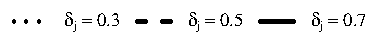
\includegraphics{LegendMarginal}

 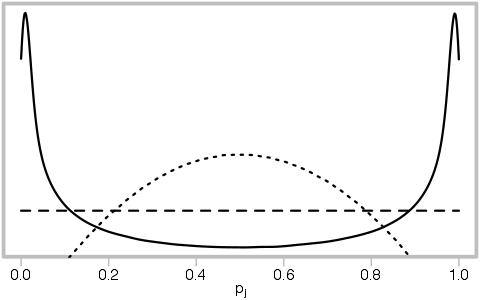
\includegraphics[width= 0.55\textwidth]{Marginals}
   \caption{The marginal distribution of $p_j$ under different levels of $\delta_j$. The more the expert knows, i.e. the higher $\delta_j$ is, the more the probability forecasts are concentrated around the extreme points 0.0 and 1.0.}
\label{marginals}
\end{figure}


\section{Probability Extremization}
\label{extremization}
%\textcolor{red}{Write about extremization wrt average probability}
The best in-principle forecast given the knowledge of $N$ experts is $P(X_{S} > 0 |  \mathcal{F}')$, where $\mathcal{F}' = \mathcal{F}_1 \cup \dots \cup \mathcal{F}_N$. This aggregate, however, assumes knowledge of the union of the information sets. Given that this union is almost always unattainable due to company confidentiality or the experts' inability to specify the knowledge that ultimately leads to their opinions (\cite{dawid1995coherent}), the best aggregate probability that can be realistically hoped for is  $\P(X_{S} > 0 | p_1, \dots, p_N)$. This section derives this aggregator under the partial information model and then uses it to analyze extremization.  In this paper extremization is understood as an increase in the strength of the belief indicated by the probability forecast. Therefore a probability $p$ for a binary event is extremized by $p'$ if $p'$ is closer to $0$ when $p \leq 0.5$ and closer to $1$ when $p \geq 0.5$.  


To derive the partial information aggregator, let $\boldsymbol{X}$ be a column vector of length $N$ such that $X_j = X_{I_j}$ for $j = 1, \dots, N$. If $\Sigma_{22}$ is a coherent overlap structure and $\Sigma_{22}^{-1}$ exists, then $X_{S} | \boldsymbol{X} \sim \mathcal{N}(\bar{\mu}, \bar{\Sigma})$, where
\begin{align}
\bar{\mu} &= \mu_1 + \Sigma_{12} \Sigma_{22}^{-1} (\boldsymbol{X} - \boldsymbol{\mu}_2) =  \Sigma_{12} \Sigma_{22}^{-1} \boldsymbol{X} \label{condMu}
\end{align}
and
\begin{align}
 \bar{\Sigma}&= \Sigma_{11} - \Sigma_{12} \Sigma_{22}^{-1} \Sigma_{21} =1 - \Sigma_{12} \Sigma_{22}^{-1} \Sigma_{21}  \label{condSigma}
\end{align}
These expression can be derived directly from the formulas of the conditional multivariate Gaussian distribution (see, e.g., Result 5.2.10 on p. 156 in \cite{ravishanker2001first}). The result is the following class of probability aggregators indexed by $\Sigma_{22}$.
\begin{align}
\P\left(A  | \boldsymbol{X}\right)  = \P\left(X_{S} > 0 | \boldsymbol{X}\right) &= \Phi\left( \frac{\Sigma_{12} \Sigma_{22}^{-1} \boldsymbol{X}}{\sqrt{1 - \Sigma_{12} \Sigma_{22}^{-1} \Sigma_{21}}}\right) \label{GeneralAggregator}
%&= \Phi\left( \frac{\boldsymbol{1}_{N}'  \Sigma_{22}^{-1} \Phi^{-1}(\boldsymbol{p})}{\sqrt{1 - \boldsymbol{1}_{N}' \Sigma_{22}^{-1} \boldsymbol{1}_{N}}}\right)
\end{align}
%This aggregator and the distribution of $\boldsymbol{p} = (p_1, p_2, \dots, p_N)$, as is induced by (\ref{NExperts}), form a consistent pair 

To link this with extermination, collect all probit-forecasts into a vector $\boldsymbol{P} = (P_{I_1} P_{I_2} \dots P_{I_N})'$, denote the average probit-forecast with $\bar{P} = \left( \sum_{j=1}^N P_{I_j} \right)/N$, and use $\alpha$ to represent the amount of extremization that the partial information aggregator (\ref{GeneralAggregator}) performs for $\bar{P}$. Then,
\begin{align}
\alpha \bar{P}&=  \frac{\Sigma_{12} \Sigma_{22}^{-1} \boldsymbol{X}}{\sqrt{1 - \Sigma_{12} \Sigma_{22}^{-1} \Sigma_{21}}}  &\Leftrightarrow&& \alpha  = \frac{N \Sigma_{12} \Sigma_{22}^{-1} \boldsymbol{X}}{\left(\boldsymbol{1}_N' \boldsymbol{P} \right) \sqrt{1 - \Sigma_{12} \Sigma_{22}^{-1} \Sigma_{21}}} \label{alpha}
\end{align}
The partial information aggregate extremizes $\bar{P}$ when $\alpha$ is greater than $1$. In the contrary, when $\alpha$ is less than 1, the partial information aggregate reverse-extremizes $\bar{P}$. Even though this paper focuses on extremization of the average probit forecast, the discussion can be easily applied to the average logit-forecast by recalling that $\text{logit}(p_i) \approx \Phi^{-1}(p_i)/\sqrt{\frac{\pi}{8}}$. Therefore the amount of extremization that the partial information aggregator performs for the average logit-forecast is $\sqrt{\frac{\pi}{8}} \approx 0.627$ times $\alpha$.  


As the extremizing factor $\alpha$ is not necessarily greater or equal to 1, the partial information aggregator (\ref{GeneralAggregator}) does not always yield an extremized probability. A case-by-case analysis reveals that the aggregator extremizes most of the time. Therefore it seems more prudent to focus the discussion on cases that do not lead to extremization. The following two examples illustrate two main sources of reverse-extremization. For the sake of clarity, the examples involve only two experts. 

%\textcolor{red}{EXPLAIN THAT THE AGGREGATE IS OFTEN MORE EXTREME THAN THE GROUP OR AT LEAST CAN BE OUTSIDE. CITE PAGES SECOND PAPER.}


\begin{example}
\label{Example1}
\textbf{Dominating Expert.} This example illustrates that the amount of extremization can be driven by an expert whose information forms a superset of information. To make this more concrete, consider the following setup.
\begin{align*}
\Sigma_{22} =  \left(\begin{array}{c c}
0.20 & 0.20\\
0.20 & 0.40 \\
 \end{array}\right)
  && 
  \begin{array}{l l}
X_{I_1} =& -0.80\\
X_{I_2} =& 0.30
 \end{array}
\end{align*}
The probability forecasts in this example are $p_1 = 0.19$ and $p_2 = 0.65$, the average probability is $\bar{p} = 0.42$, and the average probit forecast (transformed to probability space) is $\Phi(\bar{P}) = 0.40$. 
The partial information aggregate is $0.65$.  Given that this is more than 0.5 while $\bar{p}$ and $\Phi(\bar{P})$ are less than 0.5, the extremizing constant is negative. To understand this result, notice that expert $E_2$ knows everything that expert $E_1$ knows. Therefore $E_1$ does not provide any new information and can be ignored. The partial information aggregate is exactly the same as the probability forecast made by $E_2$. Given that only the partial information aggregator is able to take into account overlap information, its aggregate can differ radically from the average probability and probit-forecast when the experts share information.
\end{example}

By varying the overlap coefficient $\rho$ in Example \ref{Example1}, it is possible to establish any qualitative relationship between the partial information aggregate and the other two aggregators. Therefore no single extremization rule can always hold, and inferring the information distribution among the experts is highly important. Estimating the information structure, however, is not in the scope of this paper and is hence left for future work. Before describing the second source of reverse-extremization, it is helpful to introduce the class of non-overlapping information structures. 

\subsection{Non-overlapping Information}
\label{nonoverlap}
This section assumes that the experts' information sets do not overlap, i.e.   $|I_{i} \cap I_{j}| = \emptyset$ for all $i \neq j$. The resulting information structure is diagonal.  That is,
% $\rho \in [\max \{(N-T)/(T(N-1)), 0\},1] = A_\rho$. 
\begin{align*}
\left(\begin{matrix} X_{S} \\ X_{I_1}\\ \vdots \\ X_{I_N} \end{matrix}\right) &\sim \mathcal{N}\left( 
 \boldsymbol{0}, \left(\begin{matrix} 
\Sigma_{11} & \Sigma_{12}\\
\Sigma_{21} & \Sigma_{22}\\
 \end{matrix}\right) 
 =
 \left(\begin{array}{c|cccc}
1 & \delta_1 & \delta_2 & \dots & \delta_N  \\ \hline
\delta_1 & \delta_1 &0 & \dots & 0   \\ 
\delta_2 & 0 & \delta_2 & \dots & 0  \\ 
\vdots & \vdots & \vdots & \ddots & \vdots  \\ 
\delta_N & 0 & 0 & \dots & \delta_N\\ 
 \end{array}\right)\right),
\end{align*}
%where the super-script $(no)$ on $\Sigma_{22}$ emphasizes that this information structure is non-overlapping and hence different from the fully general structure described in (\ref{NExperts}). The other three blocks of the covariance matrix are the same as in (\ref{NExperts}). 
The information structure $\Sigma_{22}$  is coherent if and only if $\sum_{j=1}^N \delta_j \leq 1$ with all $\delta_j \in [0,1]$. The resulting aggregator is 
\begin{align}
\P\left(X_{S} > 0 | \boldsymbol{X}\right) &= \Phi\left( \frac{\sum_{j=1}^N X_{I_j}}{\sqrt{1 - \sum_{j=1}^N \delta_j}}\right) \label{VotingAggre}
\end{align}
This aggregator can be described in two steps: The first step is voting where votes are weighted according to the importance of the experts' private information. This step is performed by the summation in the numerator. If this sum falls below $0.0$ (or above $0.0$), the consensus believes that the event will not happen (or will happen). The second step is performed by the denominator that extremizes the experts' belief according to the total amount of information in the group. For instance, if the experts know all the information, i.e. $\sum_{j=1}^N \delta_j = 1$, their vote deterministically indicates whether the event $A$ happens or not. These steps do not necessarily lead to extremization. This shown in the next example that discusses the second source of reverse-extremization.

\begin{example}
\label{KeyInfo}
\textbf{Highly Influential Information.} This example illustrates that the amount of extremization can be driven by a highly influential piece of information. To make this more specific, consider the following setup.
\begin{align*}
\Sigma_{22} =  \left(\begin{array}{c c}
0.05 & 0.00\\
0.00 & 0.90 \\
 \end{array}\right)
  && 
  \begin{array}{l l}
X_{I_1} =& 0.50\\
X_{I_2} =& -0.25
 \end{array}
\end{align*}
The probability forecasts in this example are $p_1 = 0.70$ and $p_2 = 0.21$, the average probability is $\bar{p} = 0.46$, and the average probit forecast (transformed to probability space) is $\Phi(\bar{P}) = 0.44$.  The partial information aggregate is $0.87$. Therefore the extremizing constant is negative. As the information structure is diagonal, the partial information aggregate resembles voting that gives each $X_{I_j}$ equal weight despite how much the corresponding expert knows. The consensus is that the event will happen. Given that the experts know 95\% of the information, their consensus belief is extremized heavily leading to a final aggregate of $0.87$. The other two aggregates fall below $0.5$ because they weight $E_2$'s information much more than $E_1$'s information.
\end{example}

Example \ref{KeyInfo} illustrates that the partial information aggregate can be outside the convex hull of the experts' probability forecasts. Therefore it is appropriate for combining interpreted forecasts (\cite{parunak2013characterizing}). Given that the non-overlapping information structure excludes the possibility of a dominating expert, aggregator (\ref{VotingAggre}) can be expected to extremize in the absence of highly influential information. 
% It is possible to show that the aggregator (\ref{VotingAggre}) always extremizes the probit forecast when each $X_{I_j}$ falls on the same side of zero; that is, when there is no highly influential piece of information. 
% 
One version of this statement is given in the following observation.
 
\begin{observation}
\label{positiveThmVote}
Under the non-overlapping information structure, the extremizing factor, $\alpha$, is greater or equal to $1$ if either $X_{I_j} \geq 0$ or  $X_{I_j} \leq 0$, or equivalently $p_j \geq 0.5$ or $p_j \leq 0.5$ simultaneously for all $j = 1, \dots, N$. 
\end{observation}
\begin{proof} 
Let $\boldsymbol{d} = \frac{1}{N}\left((1-\delta_1)^{-1/2}, (1-\delta_2)^{-1/2}, \dots, (1-\delta_N)^{-1/2}\right)'$. Assume without loss of generality that $\bar{P} > 0$. Then the average probit forecast is extremized if
\begin{align}
 \bar{P}&\leq  \frac{\sum_{j=1}^N X_{I_j}}{\sqrt{1 - \sum_{j=1}^N \delta_j}} &\Leftrightarrow&& 0 \leq  \left(  \left(1 - \sum_{j=1}^N \delta_j \right)^{-1/2} \boldsymbol{1}_N - \boldsymbol{d}' \right) \boldsymbol{X} \label{votingproof}
\end{align}
 As $N (1-\delta_j)^{1/2} \geq \left(1 - \sum_{j=1}^N \delta_j \right)^{1/2}$ for all $j = 1, \dots, N$, all the elements of $$\left(1 - \sum_{j=1}^N \delta_j \right)^{-1/2} \boldsymbol{1}_N - \boldsymbol{d}' $$ are non-negative. Therefore the right hand side of (\ref{votingproof}) is always non-negative. 
\end{proof}
The next section discusses a class of information structures that is unaffected by both sources of reverse-extremization. The corresponding aggregator always extremizes the average probit-forecast. 

\subsection{Compound Symmetric Information}
\label{compound}

This section assumes that the experts' information sets have the same size and that the amount of overlap between any two information sets is constant, i.e.  $|I_{1}| =  \dots = |I_{N}|$ and $|I_{i} \cap I_{j}| = |I_{h} \cap I_{k}|$ for all $i \neq j$ and $h \neq k$. In other words, each expert knows and shares the same amount with every other expert. Therefore the experts are exchangeable, and no single expert can dominate. The resulting information structure is compound symmetric. That is,
% $\rho \in [\max \{(N-T)/(T(N-1)), 0\},1] = A_\rho$. 
\begin{align*}
\left(\begin{matrix} X_{S} \\ X_{I_1}\\ \vdots \\ X_{I_N} \end{matrix}\right) &\sim \mathcal{N}\left( 
 \boldsymbol{0}, \left(\begin{matrix} 
\Sigma_{11} & \Sigma_{12}\\
\Sigma_{21} & \Sigma_{22}\\
 \end{matrix}\right) 
 =
 \left(\begin{array}{c|cccc}
1 & \delta & \delta & \dots & \delta  \\ \hline
\delta & \delta &\lambda\delta & \dots & \lambda\delta   \\ 
\delta & \lambda\delta & \delta & \dots & \lambda\delta  \\ 
\vdots & \vdots & \vdots & \ddots & \vdots  \\ 
\delta & \lambda\delta & \lambda\delta & \dots & \delta\\ 
 \end{array}\right)\right),
\end{align*}
%where the super-script $(cs)$ emphasizes that this information structure is compound symmetric and hence different from the fully general structure described in (\ref{NExperts}). Only the top-left block of the covariance matrix is the same as in (\ref{NExperts}). 
The amount of information known by each expert is denoted with $\delta \in [0,1]$. The value of $\lambda$ is the proportion of the known information that is shared between any two experts.  This minor change of parametrization was made for the sake of simplifying some of the following expressions. To ensure that $\Sigma_{22}$ is coherent, a domain restriction must be placed on $\lambda$. First, the upper bound for $\lambda$ is $1$ because under any combination of $\delta$ and $N$ it is possible that all experts know the exact same information. Second, to derive the lower bound, observe that information overlap is unavoidable if $\delta > 1/N$. The minimum sharing occurs when all information is either shared or private. In other words, if $\delta > 1/N$ and $I_{i} \cap I_j = I$ and $|I| =  \lambda \delta$ for all $i \neq j$, the minimum sharing occurs when $\lambda\delta + N(\delta - \delta\lambda) = 1$. Solving for $\lambda$ gives the desired lower bound. The domain restriction on $\lambda$ then becomes
\begin{align}
\lambda &\in \left[  \max \left\{ \frac{N-\delta^{-1}}{N-1}, 0\right\}, 1 \right] \label{rhoDomain}
\end{align}
The quantity  $\lambda\delta + N(\delta - \delta\lambda)$ also describes the maximum information coverage of the $N$ experts, i.e. $\max | I_1 \cup I_2 \cup \dots \cup I_N| = \lambda\delta + N(\delta - \delta\lambda)$. 

In practice the values of $\delta$ and $\lambda$ can be estimated via the maximum likelihood method. To make this more explicit, observe that $\boldsymbol{P} \sim \mathcal{N}_N\left(\boldsymbol{0}, \Sigma_{22} (1-\delta)^{-1}\right)$ and that the Jacobian for the map $\boldsymbol{P} \to \Phi\left(\boldsymbol{P}\right)$ is
\begin{eqnarray*}
J(\boldsymbol{X}) &=& (2\pi)^{-N/2} \exp \left( - \frac{\boldsymbol{P}' \boldsymbol{P}}{2}   \right) 
\end{eqnarray*}
If $h(\boldsymbol{P})$ denotes the multivariate Gaussian density of $\boldsymbol{P}$,  
%by the Inverse Function Theorem 
the density for  $\boldsymbol{p} = (p_1, p_2, \dots, p_N)$ is 
\begin{eqnarray*}
 f\left(\boldsymbol{p} | \delta, \lambda \right) &=& h(\boldsymbol{P}) J(\boldsymbol{P})^{-1} \bigg|_{\boldsymbol{P} = \Phi^{-1}(\boldsymbol{p})}\\
%&=& \frac{(1-\delta)^{N/2}}{\sqrt{ |\Sigma_{22}|}} \exp\left( -\frac{1}{2} \boldsymbol{P}' (1-\delta)\Sigma_{22}^{-1} \boldsymbol{P} + \frac{\boldsymbol{P}' \boldsymbol{P}}{2}   \right)\\
&=& \frac{(1-\delta)^{N/2}}{\sqrt{ \left|\Sigma_{22}\right|}} \exp\left( -\frac{1}{2} \Phi^{-1}(\boldsymbol{p})' \left( (1-\delta) \left(\Sigma_{22}\right)^{-1} - I_N \right) \Phi^{-1}(\boldsymbol{p})  \right) 
\end{eqnarray*}
where $\Phi^{-1}(\boldsymbol{p}) =  (\Phi^{-1}(p_1), \Phi^{-1}(p_2), \dots, \Phi^{-1}(p_N))$. 
%Given that $\Sigma_{22}$ can be written in the form  $\Sigma_{22} = I_N (\delta-\lambda\delta) + J_{N \times N} \lambda\delta$
The inverse of $\Sigma_{22}$  is
\begin{align}
\left(\Sigma_{22}\right)^{-1} = I_N \left(\frac{1}{\delta-\lambda\delta} \right) - J_{N \times N} \frac{\lambda}{(1-\lambda)\delta(1+(N-1) \lambda)} \label{inverse},
\end{align}
where $J_{N \times N}$ is a matrix of ones with $N$ columns and rows (see the supplementary material of \cite{dobbin2005sample} for the proof of this fact).  According to p. 32 in \cite{rao2009linear}, the determinant of $\Sigma_{22}$ is
\begin{align*}
%| \Sigma_{22}| = (\delta - \lambda\delta)^N \left(1+\frac{N \delta \lambda}{\delta - \delta\lambda} \right),
\left| \Sigma_{22}\right| = (\delta(1- \lambda))^N \left(1+\frac{N \lambda}{1 - \lambda} \right),
\end{align*}
The maximum likelihood estimates of $\delta$ and $\lambda$ are then obtained from
\begin{align}
(\hat{\delta}, \hat{\lambda}) =& \argmax_{\lambda, \delta} \log  f\left(\boldsymbol{p}| \delta, \lambda \right), \label{MLE}\\
& \text{s.t. } \nonumber \delta \in [0,1] \text{ and } \lambda \in \left[  \max \left\{ \frac{N-\delta^{-1}}{N-1}, 0\right\}, 1 \right]
\end{align}
Unfortunately, (\ref{MLE}) cannot be solved analytically. However, a simple grid-search can be used to find the estimates very efficiently. 

%\begin{align*}
%(\hat{\delta}, \hat{\lambda}) &= \argmax_{\lambda, \delta}  - \frac{N}{2} \log (\delta - \lambda\delta) - \frac{1}{2} \log \left(1+\frac{N \delta \lambda}{\delta - \delta\lambda} \right) -\frac{1}{2} \boldsymbol{X}' \left( I_N \left(\frac{1}{\delta-\lambda\delta} \right) - J_{N \times N} \frac{\lambda}{(1-\lambda)\delta(1+(N-1) \lambda)}  \right) \boldsymbol{X}
%\end{align*}




%Recall that if $X_{I_j} \sim \mathcal{N}(0,1)$, then $\Phi(X_{I_j})$ is uniform on $[0,1]$. Therefore, if $\delta_j = 1$, the marginal distribution of $p_j = \Phi(X_{I_j})$ is uniform on $[0,1]$. If this does not hold empirically, it is a sign that the model cannot be correct on the micro-level. If $X_{I_j}$ appears more (respectively less) concentrated about $0.5$, then the model can be adjusted by changing $\delta_{j}$ to a smaller fraction. 


%Assuming no further prior information on overlap structure, the expected amount of information held by the group is WHAT IS THIS?

The aggregator under the compound symmetric information structure can be derived by applying (\ref{inverse}) to the general formulas (\ref{condMu}) and (\ref{condSigma}). The resulting conditional mean and variance are 
%By the conditional multivariate normal results, we have that 
%\begin{align*}
%\bar{\mu} &= \mu_1 + \Sigma_{12} \Sigma_{22}^{-1} (\boldsymbol{X} - \boldsymbol{\mu}_2)\\
% &= \Sigma_{12} \Sigma_{22}^{-1} \boldsymbol{X} \\
% \\
% \bar{\Sigma}&= \Sigma_{11} - \Sigma_{12} \Sigma_{22}^{-1} \Sigma_{21}\\
%&=1 - \Sigma_{12} \Sigma_{22}^{-1} \Sigma_{21}
%\end{align*}
%
%%(see \url{http://linus.nci.nih.gov/techreport/DobbinSimonAppendix.pdf} for this). 
%Hence the off-diagonals of $\Sigma_{22}^{-1}$ are 
%\begin{align*}
%\frac{\lambda\delta}{(\lambda\delta-\delta)((N-1)\lambda\delta +\delta)}
%\end{align*}
%and the diagonals are
%\begin{align*}
%\frac{(2-N)\lambda\delta -\delta}{(\lambda\delta-\delta)((N-1)\lambda\delta +\delta)}
%\end{align*}
%The conditional mean can be derived as
%\begin{align*}
%\Sigma_{22}^{-1} &= \frac{1}{(\lambda\delta-\delta)((N-1)\lambda\delta +\delta)}
% \left(\begin{matrix} 
%(2-N)\lambda\delta -\delta & \lambda\delta & \dots & \lambda\delta \\ 
%\lambda\delta & (2-N)\lambda\delta -\delta & \dots & \lambda\delta \\ 
%\vdots & \vdots &  \ddots & \vdots \\ 
%\lambda\delta & \lambda\delta & \dots & (2-N)\lambda\delta -\delta  \\ 
% \end{matrix}\right)\\
% \Sigma_{12} \Sigma_{22}^{-1} &= \frac{\delta}{(\lambda\delta-\delta)((N-1)\lambda\delta +\delta)} \left( \begin{matrix} \lambda\delta -\delta &  \dots & \lambda\delta -\delta \end{matrix} \right)\\
% \Sigma_{12} \Sigma_{22}^{-1} \boldsymbol{X} &= \frac{\delta}{(\lambda\delta-\delta)((N-1)\lambda\delta +\delta)} (\lambda\delta -\delta) \sum_{j=1}^N X_j \\
%&= \frac{\delta(\lambda\delta -\delta)}{(\lambda\delta-\delta)((N-1)\lambda\delta +\delta)}  \sum_{j=1}^N X_j \\
%&= \frac{\delta}{(N-1)\lambda\delta +\delta}  \sum_{j=1}^N X_j \\
\begin{align*}
\bar{\mu} = \frac{1}{(N-1)\lambda +1}  \sum_{j=1}^N X_j 
% \bar{\Sigma} &= 1 -  \Sigma_{12} \Sigma_{22}^{-1}\Sigma_{21} \\
% &= 1  - \frac{\delta^2}{(\lambda\delta-\delta)((N-1)\lambda\delta +\delta)} N(\lambda\delta -\delta)\\
% &= 1  - \frac{\delta^2N}{(N-1)\lambda\delta +\delta} \\
&&  \bar{\Sigma} = 1  - \frac{\delta N}{(N-1)\lambda +1} 
\end{align*}
Therefore the  aggregator becomes
\begin{align}
\P\left(X_S > 0 | \boldsymbol{X}\right) &=\Phi\left(\frac{\frac{1}{(N-1)\lambda +1} \sum_{j=1}^N X_{I_j} }{\sqrt{1- \frac{N\delta}{(N-1)\lambda +1} }}  \right) \label{CompoundAggre}
\end{align}
%It is crucial to notice that this aggregator can learn the amount of extremization without a separate training set. Therefore it can be applied to a wide range of applied problems. 
Equating this with $\alpha \bar{P}$ results in the following extremizing factor.
\begin{align}
%\alpha \bar{X}  &=  \frac{\frac{1}{(N-1)\lambda +1} \sum_{j=1}^N X_j }{\sqrt{T- \frac{N}{(N-1)\lambda +1} }}\\
%\alpha &= \frac{\frac{1}{(N-1)\lambda +1} \sum_{j=1}^N X_j }{\bar{X} \sqrt{T- \frac{N}{(N-1)\lambda +1} }}\\
\alpha &= \frac{\frac{N\sqrt{1-\delta}}{(N-1)\lambda +1}}{\sqrt{1- \frac{N\delta}{(N-1)\lambda +1} }} \label{CompoundAlpha}
% &= \frac{\frac{N}{(N-1)\lambda +1}}{\sqrt{1-\delta  \left( \frac{N}{(N-1)\lambda +1}  \right)}} \\
% &= \frac{\gamma}{\sqrt{1-\delta\gamma}},
% &= \frac{N}{\sqrt{((N-1)\lambda +1)^2 (T- \frac{N}{(N-1)\lambda +1} )}}\\
% &= \frac{N}{\sqrt{((N-1)\lambda +1)^2T- N((N-1)\lambda +1) )}}
\end{align}
%where 
%\begin{align*}
%\gamma &= \frac{N}{(N-1)\lambda +1}\\
%&= \left( \frac{1}{(N-1)\lambda +1} \right) N\\
%\end{align*}
%WHAT IS GAMMA? Given that 
%\begin{align*}
%\gamma \delta &\leq 1\\
%% \frac{N \delta}{(N-1)\lambda +1}  &\leq& 1\\
% \frac{N\delta - 1}{N-1}  &\leq \lambda,
%\end{align*}
Given that the square-root is not defined for negative values,  it must be required that
\begin{align}
1- \frac{N\delta}{(N-1)\lambda +1}  &\geq 0 &\Leftrightarrow&& \lambda \geq \frac{N\delta - 1}{N-1} \label{rhoDomain2}
\end{align}
Contrast this with former domain restriction (\ref{rhoDomain}) and observe that both $N\delta - 1$ and $N - \delta^{-1}$ are negative when $\delta < 1/N$. Given that $N\delta - 1 > N - \delta^{-1}$ only when $\delta < 1/N$, the latter restriction (\ref{rhoDomain2}) is redundant and can be ignored. 

Expression (\ref{CompoundAlpha}) is positively associated with $N$ and $\delta$ but negatively associated with $\lambda$. Therefore the amount of extremization is positively associated with the total amount of information in the group of experts. The amount of extremization cannot be driven by highly influential information because (\ref{CompoundAlpha}) does not depend on $\boldsymbol{X}$. Therefore, given that the amount of extremization is unaffected by both sources of reverse-extremization, it is not surprising that the aggregator (\ref{CompoundAggre}) always extremizes. This is stated more formally in the following observation.

\begin{observation}
\label{positiveThm}
Under the compound symmetric information structure, the extremizing factor $\alpha$ is always greater or equal to 1. 
\end{observation}
\begin{proof} 
For a given $\delta$, the extremizing constant $\alpha$ is minimized when $(N-1)\lambda +1$ is maximized. This happens at $\lambda = 1$. Plugging this into (\ref{CompoundAlpha}) gives
\begin{align*}
\alpha &= \frac{\frac{N\sqrt{1-\delta}}{(N-1)\lambda +1}}{\sqrt{1- \frac{N\delta}{(N-1)\lambda +1} }}  \geq \frac{\sqrt{1-\delta}}{\sqrt{1-\delta }} = 1
\end{align*}
\end{proof}




%As $\frac{N}{(N-1)\lambda +1} \in [1, N]$, this quantity can be thought of as the amount of knowledge that the group knows. Therefore $\alpha$ is a ratio of the amount of knowledge known and the amount of knowledge that is unknown to the group. This makes intuitively sense because if the group knows almost all of $T$, then their average should be heavily extremized.
% If the group of experts is large, then $N-1 \approx N$ and 
%\begin{align*}
%\alpha &= \frac{\frac{N}{N\lambda +1} }{\sqrt{T- \frac{N}{N\lambda +1} }}
%\end{align*}
%
%
%
%\begin{figure}[hbt!]
%\begin{minipage}[t]{0.33\textwidth}
%\centering
%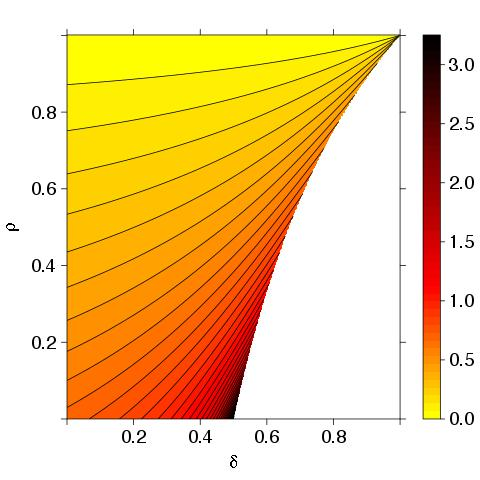
\includegraphics[width=\textwidth, height = \textwidth]{ExtremeN2.jpeg}
%\caption{N = 2}
%\label{ExtremeN5}
%\end{minipage}
%\begin{minipage}[t]{0.33\textwidth}
%\centering
%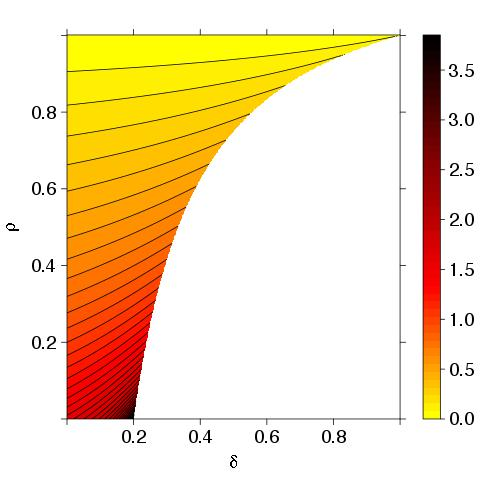
\includegraphics[width=\textwidth, height = \textwidth]{ExtremeN5.jpeg}
%\caption{N = 5}
%\label{ExtremeN10}
%\end{minipage}
%\begin{minipage}[t]{0.33\textwidth}
%\centering
%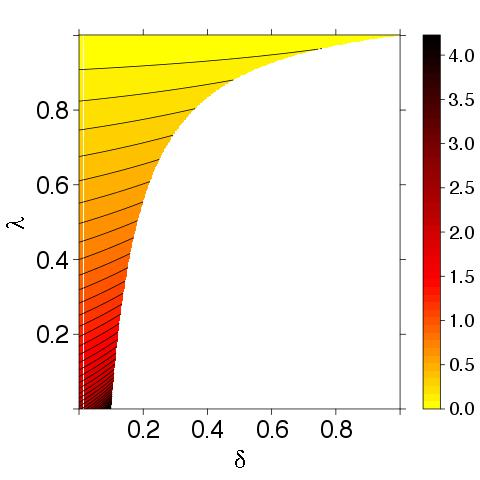
\includegraphics[width=\textwidth, height = \textwidth]{ExtremeN10.jpeg}
%\caption{N = 10}
%\label{ExtremeN30}
%\end{minipage}
%\end{figure}


\begin{figure}
        \centering
        \begin{subfigure}[b]{0.45\textwidth}
                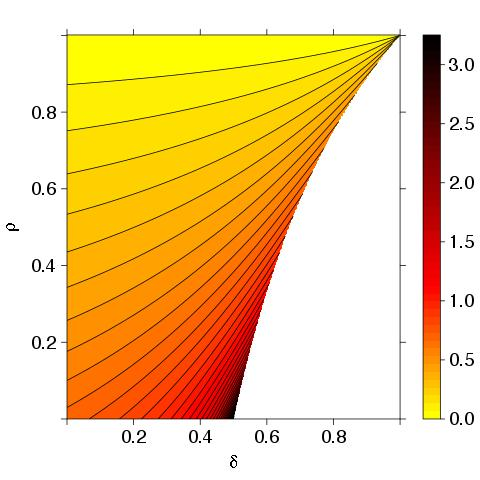
\includegraphics[width=\textwidth]{ExtremeN2.jpeg}
\caption{N = 2}	
\label{ExtremeN5}
        \end{subfigure}%
        ~ %add desired spacing between images, e. g. ~, \quad, \qquad etc.
          %(or a blank line to force the subfigure onto a new line)
%        \begin{subfigure}[b]{0.32\textwidth}
%                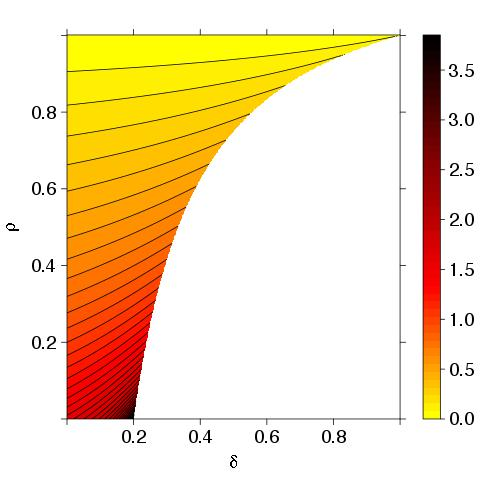
\includegraphics[width=\textwidth]{ExtremeN5.jpeg}
%\caption{N = 5}
%\label{ExtremeN10}
%        \end{subfigure}
        ~ %add desired spacing between images, e. g. ~, \quad, \qquad etc.
          %(or a blank line to force the subfigure onto a new line)
        \begin{subfigure}[b]{0.45\textwidth}
                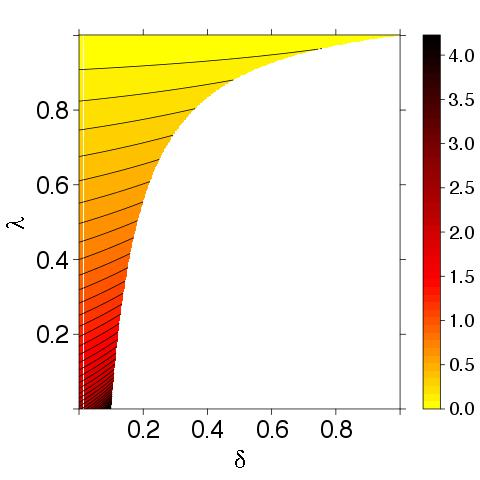
\includegraphics[width=\textwidth]{ExtremeN10.jpeg}
\caption{N = 10}
\label{ExtremeN30}
        \end{subfigure}
        \caption{ The amount of log-extremization $\log(\alpha)$ under different combinations of $N$ (the number of experts), $\delta$ (the amount of information known by one expert), and $\lambda$ (the amount of information shared by any two experts).}
\end{figure}



Because the extremizing factor (\ref{CompoundAlpha}) depends only on three intuitive parameters, it can be analyzed graphically. Figures \ref{ExtremeN5} and \ref{ExtremeN30} describe the amount of log-extremization $\log(\alpha)$ under different values of $\lambda, \delta$, and $N$. High values have been censored to keep the scale manageable. By Observation \ref{positiveThm} the amount of extremizing is always greater or equal to 1.0. The extremizing factor increases indefinitely towards the point $\delta = 1/N$ and $\lambda = 0$. In this case the experts' information sets form a partition of the full information. Therefore the experts know all the information. Such a group of experts can re-construct $X_S$ by simply adding up their  information. This turns aggregation into deterministic voting: if the sum of the probit-forecasts is above 0, the event $A$ materializes; else it does not. A similar observation has been made under the interpreted forecasts (\cite{hong2009interpreted}). 

 

%Moving towards the upper left corner, where $\delta = 0.0$ and $\lambda = 1.0$, decreases the amount of extremizing monotonically to $1.0$.
The amount of extremization decreases as a) the amount of information that each individual expert holds decreases ($\delta$ decreases) and/or b) the amount of shared information increases ($\lambda$ increases). Therefore the more knowledgable and diverse the group of experts is, the more their average probit-forecast should be extremized. The only exception occurs when $\lambda = 1.0$. In this case, all information is public, and the group of experts is as good as a single expert. Therefore, given that a single expert's forecast should not be extremized, $\lambda = 1.0$ always implies $\alpha = 1.0$ regardless of the value of $\delta$. 


Given that increasing $\lambda$ results in more similar probability forecasts, the value of $\lambda$ is inversely proportional to the variance of the forecasts. Therefore, if more extremizing is viewed as increased confidence in the final outcome, higher variance in the probability forecasts can be considered helpful. Contrast this with the classical measurement error model where increased variance is typically considered harmful. This reversal of the effect is an important property of the interpreted forecasts (\cite{hong2009interpreted}). 


From Figures \ref{ExtremeN5} and \ref{ExtremeN30} it is clear that the feasible set of $(\delta, \lambda)$-values becomes smaller as $N$ increases. This limitation arises from assuming a compound symmetric overlap structure. Having many experts, each with a considerable amount of information, simply leads to unavoidable overlap in the information sets. From the domain restriction (\ref{rhoDomain}), it is clear that $\lambda \to 1$ as $N \to \infty$. Therefore in the limit the group of experts is equivalent to a single expert. This observation clearly does not reflect the real-world. When $N = 2$, on other hand, the compound symmetric overlap is almost fully general. Therefore assuming a compound symmetric information structure can be appropriate for small numbers of experts but becomes overly restrictive as more experts enter the group. 


\section{Discussion}

% What did we learn from this ?

% 1. In the real world there does not seem to be the two sources of reverse-extremization. X
% 2. Illustrated that parameters can be estimated X
% 2b. Future work: learning about overlap structures X
% 3. Summarize main observations: 
% (i) extremization increases as a function of information in the group. X
% (ii) Voting works well under high diversity. 
% 4. Process can be repeated for something else besides extremization X
% 5. Limitation: Discuss optimality constraint 
% 6. The model checks with intuition. X

% 7. Overall, the procedure resembles voting. Therefore voting can be expected to work well in practice when the voters form a very knowledgable and diverse group of experts.

This paper began by introducing a partial information model for probability forecasts. The model was used to derive and study an entire class of probability aggregators that are closely linked to the actual environment of probability forecasts. As a result, many of the results aligned well with intuition.  In particular, the analysis showed that the amount of extremizing is positively associated with the total amount of information in the group of experts, and also presented two main sources of reverse-extremization: i) a dominant expert whose information forms (or at least approximates) a superset of information, and ii) highly influential information that ultimately decides the outcome of the target event. Given that many previous studies have found extremization to improve aggregate predictions in the real world, it is likely that these sources are not very common in practice. These sources were central in guiding the discussion towards the non-overlapping and compound symmetric information structures. Given that the latter is unaffected by both sources of reverse-extremization, the corresponding aggregator always extremizes. Therefore it is suitable for aggregation of expert beliefs in the absence of a separate training set.

New aggregators can also be developed by finding new ways to estimate the information structure. It seems difficult, if possible at all, to estimate the information structure in its full generality. Therefore it will be necessary to pose some constraints on the structure. Section \ref{compound} illustrated this by giving explicit instructions on how to estimate the structure under compound symmetric information. Unfortunately, this structure has poor limiting behavior. Part of our future work is to develop a class of information structures that is  both estimable and realistic for large number of experts.  A different alternative is to construct a realistic prior distribution for the information structure, update this prior to a posterior distribution via the multivariate normal likelihood function, and then marginalize the information structure with respect to its posterior distribution.  

 
 Other future directions could  remove some of the obvious limitations of the model. For instance, assuming that the experts' produce optimal probability forecasts given their private information sets may not be a realistic assumption. The experts may believe in false information, hide their true beliefs, or be biased for many other reasons. This could be expressed in the model by introducing an error term, possibly with a mean of zero, that is added to the experts' optimal forecasts. Even though adding such an error term might improve the real-world performance of resulting aggregators, it is hardly necessary in this paper as the results are conceptual. After all, the cleanest discussion follows from assuming optimal forecasts. 
 
% This assumption is natural if a subjective probability is considered logical and objectively determined by evidence (see, e.g., \cite{carnap1962logical, jeffreys1998theory, keynes2004treatise}). \cite{dawid1995coherent} also argue that an aggregator should be hesitant in involving experts' whose world views differ radically from that of the decision maker. 
% 
% They state that ``[a]t any rate, the condition has sufficient \textit{prima facie} appeal to make it worthwhile to investigate its consequences."

 
 
 


%\bibliographystyle{plain}
\bibliographystyle{plainnat}
\bibliography{biblio}		% expects file "myrefs.bib"



\end{document}
